
\chapter{Metodologia\label{chap:Metodos}}

% Resumo opcional. Comentar se não usar.
%\resumodocapitulo{resumo}


\section{Materiais}
\subsection{Hardware}
\subsubsection{Leitora RFID Impinj Speedway R420}

A Speedway R420 da fabricante Impinj é uma pequena leitora estacionária de \textit{tags} de RFID passivo. Ela é capaz de operar na faixa de frequência de 860-960 MHz, sendo que o modelo específico licenciado para o Brasil permite operações entre 902,5 e 907 MHz. Pode emitir sinais de até 32,25 dBm de potência na transmissão e é capaz de receber um sinal com a sensibilidade mínima de -80 dBm e perda de retorno de 10 dB \cite{SpeedwayRDatasheet} \cite{SpeedwayRUserManual} \cite{TG2013OliveiraERocha}. A figura \ref{fig:SpeedwayR420_first} mostra uma foto da leitora.

    \begin{figure}[H]
        \centering
        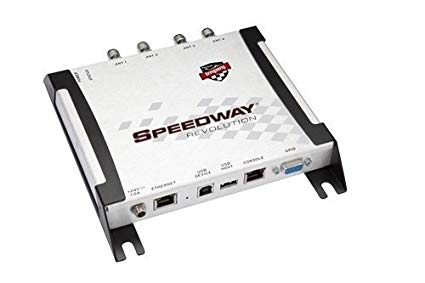
\includegraphics[width=0.55\linewidth]{figs/Metodologia/leitoraSpeedwayR420.jpg}
        \caption{Leitora Impinj Speedway R420 \cite{SpeedwayRUserManual}}
        \label{fig:SpeedwayR420_first}
    \end{figure}

 A leitora é capaz de registrar até 1100 etiquetas por segundo. Ela possui portas suficientes para o acoplamento de até 4 antenas, expansível até 32 antenas utilizando \textit{Hubs} específicos para esta aplicação. Dois protocolos são utilizados para a interface por ar: \textit{GS1/EPCglobal UHF Gen2 (ISO 18000-6C)} e \textit{RAIN RFID} \cite{SpeedwayRDatasheet}\cite{SpeedwayRUserManual}. As portas de conexão das antenas podem ser vistas na figura \ref{fig:SpeedwayR420front}.
 
     \begin{figure}[H]
        \centering
        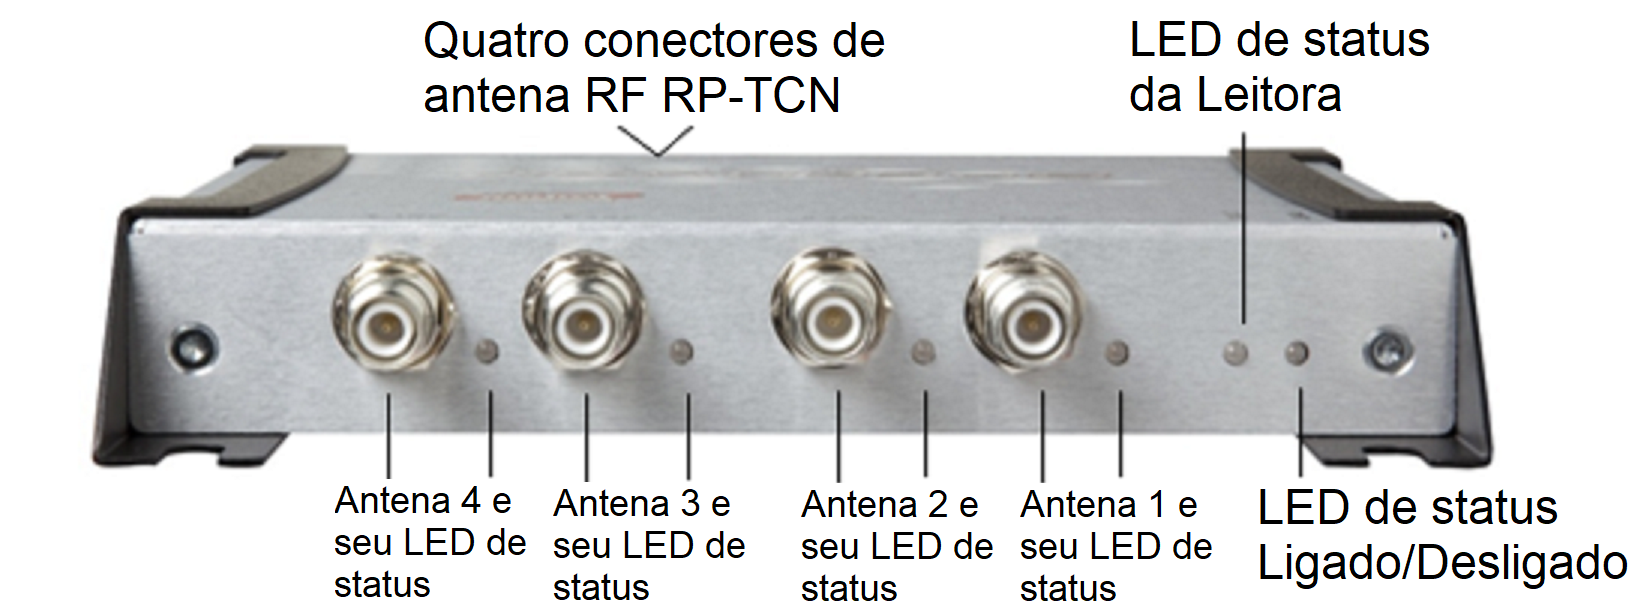
\includegraphics[width=0.6\linewidth]{figs/Metodologia/SpeedwayR420-front-view.png}
        \caption{Leitora Impinj Speedway R420 - vista frontal \cite{SpeedwayRUserManual}.}
        \label{fig:SpeedwayR420front}
    \end{figure}
 
 Existem diversas portas na parte traseira da leitora Speedway R420. Uma delas é uma porta \textit{10/100 BaseT Ethernet} para comunicação em TCP/IP. A comunicação por TCP/IP é ideal para o uso comum, utilizando os softwares comercializados pela Impinj ou por programas feitos utilizando o pacote \textit{Impinj OctaneSDK}. Além dessa porta, a comunicação pode ser feita por USB ou por comunicação serial RS-232 em um conector RJ45 para acesso ao console embarcado na leitora. As portas seriais são ideais para utilização dos pacotes \textit{Impinj LTK} de programação em baixo nível, utilizando o padrão \textit{Low Level Reader Protocol} (LLRP). Baixo nível, neste caso, implica capacidade de alterar o protocolo de operação, o modo de marcação de tempo e dos parâmetros de comando por ar\cite{GS1-LLRP}\cite{SpeedwayRUserManual}. A visão traseira da leitora é apresentada na figura \ref{fig:SpeedwayR420back}.
 
\begin{figure}[H]
    \centering
    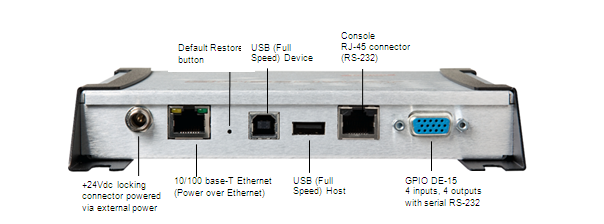
\includegraphics[width=0.6\linewidth]{figs/Metodologia/SpeedwayR420-back-view.png}
    \caption{Leitora Impinj Speedway R420 - vista traseira - Foto obtida no manual de instalação e operação da leitora \cite{SpeedwayRUserManual}.}
    \label{fig:SpeedwayR420back}
\end{figure}
 
 Existe ainda uma porta \textit{GPIO DE-15} (\textit{General Purpose Input-Output DE-15} - Porta de uso de próstio geral para entrada e saída de dados)\cite{SpeedwayRUserManual}. Ela pode ser utilizada para a configuração de comandos e gatilhos de leitura.
 
 A alimentação elétrica da leitora pode ser feita utilizando o padrão \textit{PoE} (\textit{Power over Ethernet}) \cite{SpeedwayRUserManual}, ou seja, sem a necessidade de fonte externa, apenas através do cabo Ethernet, ou então pode ser feita com uma fonte 24 volts de corrente contínua \cite{IEEE-SA-POE}. A fonte pode prover uma confiabilidade maior para operação com potências maiores, próximas ao limite de 32,25 dBm, enquanto a alimentação \textit{PoE} permite maior flexibilidade na instalação do produto, principalmente em relação à passagem de cabos e instalação de tomadas.
 
 \subsubsection{Antena RFID Impinj Threshold}
 
 A Threshold, também da fabricante Impinj, é uma antena RAIN RFID específica para detectar cruzamento de barreiras e fronteiras. O seu corpo alongado, com polarização linear paralela ao menor eixo, permite uma ampla cobertura, e a possibilidade de conectar múltiplas antenas para criar uma "cortina" de cobertura RFID \cite{AntenaThresholdDatasheet}.A antena pode ser vista na figura \ref{fig:AntenaThreshold_first} a seguir.
 
 \begin{figure}[H]
    \centering
    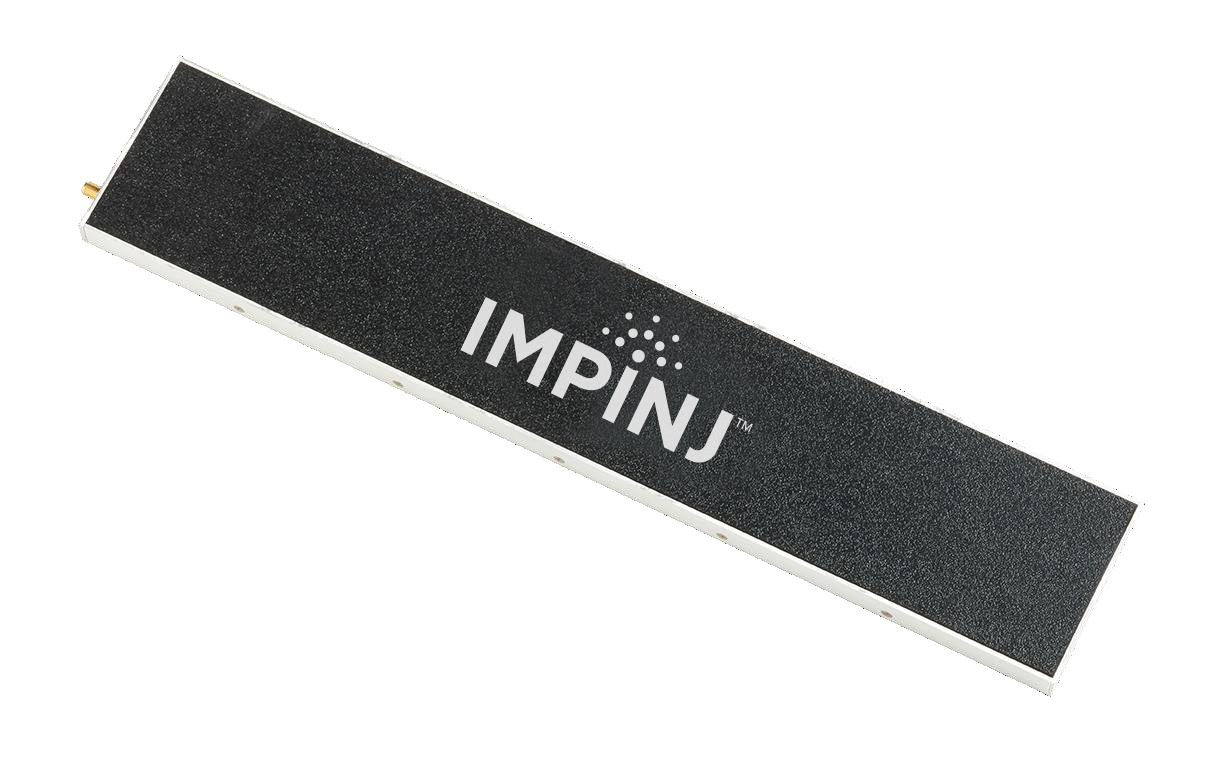
\includegraphics[width=0.5\linewidth]{figs/Metodologia/impinj_Threshold.png}
    \caption{Antena Impinj Threshold - Foto obtida no \textit{datasheet} da antena \cite{AntenaThresholdDatasheet}}
    \label{fig:AntenaThreshold_first}
\end{figure}
 
 A antena opera em duas faixas de frequência: 902-928 MHz (FCC) e 865-868 MHz (ETSI), possui um ganho de campo distante de 5.0 dBi e impedância nominal de 50 $\Omega$ \cite{AntenaThresholdDatasheet}. A antena cobre um volume elipsoidal de 3m de comprimento por 4m de largura por 3m de altura, como pode ser visto na figura \ref{fig:AntenaThresholdCobertura}.
 
  \begin{figure}[H]
    \centering
    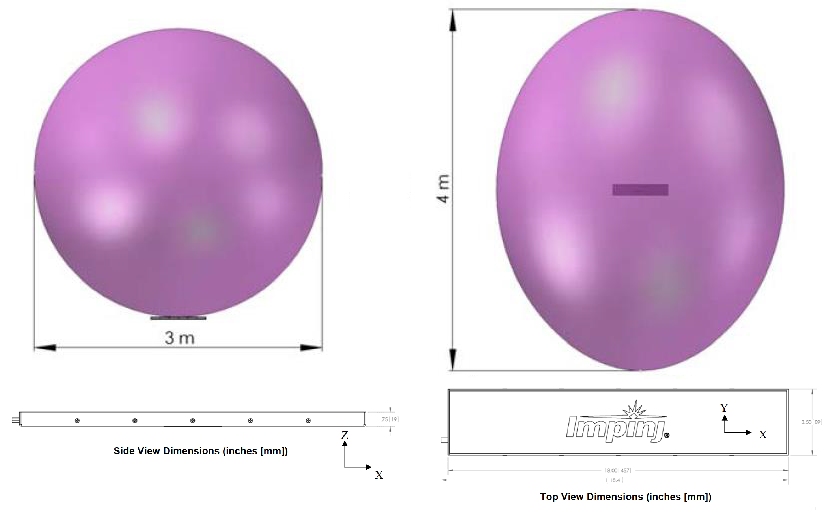
\includegraphics[width=0.6\linewidth]{figs/Metodologia/impinj_antenna_coverage.png}
    \caption{Gráfico da zona de cobertura das antenas Impinj Threshold e desenho mecânico da leitora em pontos de vista iguais aos dos desenhos de cobertura acima - Adaptado do \textit{datasheet} da antena \cite{AntenaThresholdDatasheet}}
    \label{fig:AntenaThresholdCobertura}
\end{figure}

\subsubsection{TAG utilizada no projeto}

As TAGs utilizadas são impressas em adesivos pela empresa Nycti BR. Elas utilizam chip Alien Higgs-3 RFID IC. Como características principais estão:

\begin{itemize}
    \item Banda de operação de 915-868 Mhz;
    \item Tamanho 96 X 23mm;
    \item Alcance de leitura de acordo com o fabricante de 6m (com testes empíricos feitos nas TAGs utilizadas de alcance de mais de 10m);
    \item 800-bit de memória, sendo 96 bits para armazenar o EPC - extensível até 480 bits - e 512 bits de uso de propósito geral; \cite{AlienHiggs3}
    \item ativado em baixíssimas potências de alimentação, ainda provendo excelente sinal de resposta de retroespalhamento. \cite{AlienHiggs3}
\end{itemize}

A figura \ref{fig:TAGsused} a seguir mostra as TAGs utilizadas para monitorar o trânsito das pessoas no interior dos ambientes pre-estabelecidos.

 \begin{figure}[H]
    \centering
    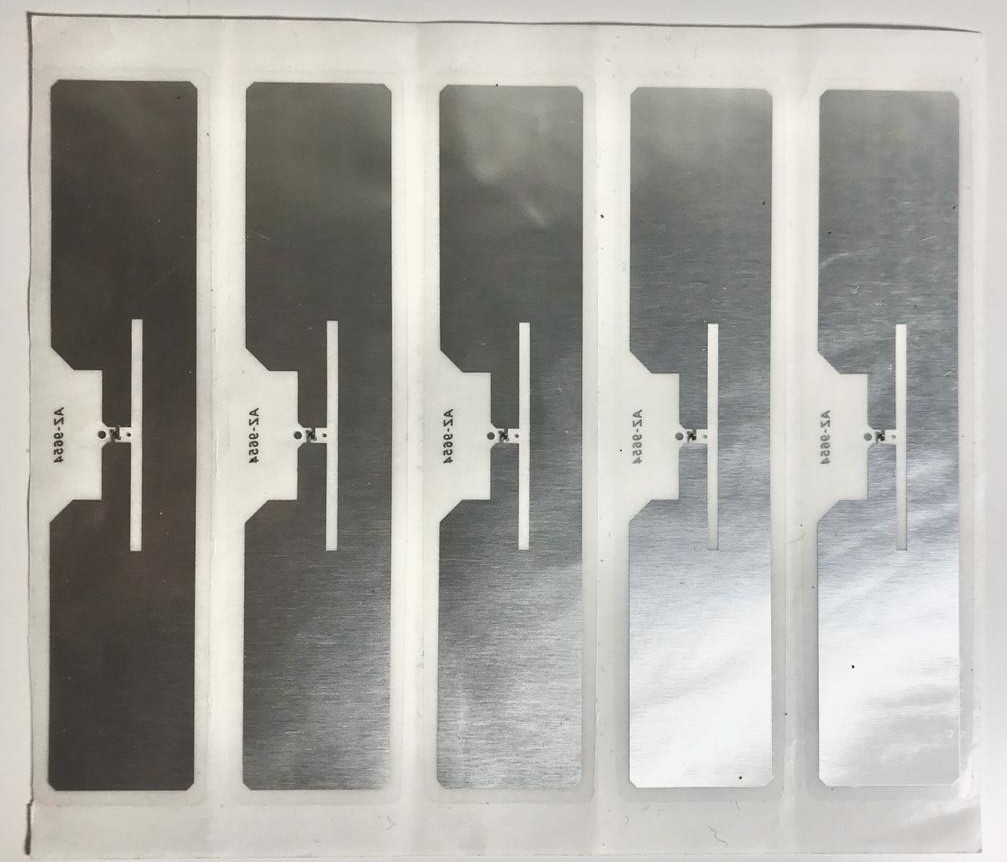
\includegraphics[width=0.8\linewidth]{figs/Metodologia/TAGsRFID.jpeg}
    \caption{TAGs utilizadas para a execução deste trabalho}
    \label{fig:TAGsused}
\end{figure}
 
 Estas TAGs mostradas na figura \ref{fig:TAGsused} foram distribuídas entre as pessoas designadas para testar o sistema criado. %TODO
 
 \subsubsection{Quantitativo}
 
 Este trabalho conta com leitoras e antenas RFID, além do espaço para trabalho e testes, gentilmente cedidos pelo Laboratório de Automação e Robótica (LARA) da UnB. No que se refere aos equipamentos, foram utilizados com os seguintes dispositivos:
 
 \begin{itemize}
     \item 3 (três) Leitoras IMPINJ Speedway R420 (cedidas pelo LARA)
     \item 6 (seis) Antenas IMPINJ Treshold (cedidas pelo LARA)
     \item 1 (um) hub DLINK 6 portas Ethernet
     \item 20 (vinte) TAGs RFID 915 MHZ
     \item cabeamento e fontes de alimentação necessários
 \end{itemize}
 
 \subsection{Software}
 
 \subsubsection{OctaneSDK}
 
 O pacote de desenvolvimento OctaneSDK para dispositivos RAIN RFID, da Impinj, foi utilizado para desenvolver a parte de software deste trabalho. O pacote possui versões para .NET e Java \cite{OctaneSDK}. O pacote para .NET foi lançado há mais tempo e possui mais versões, e, por conseguinte, mais defeitos foram corrigidos, o que torna esta implementação mais robusta do que o pacote em Java. Por esse motivo, foi escolhido para o desenvolvimento desse trabalho.
 
 \subsubsection{Visual Studio}
 
 O pacote OctaneSDK .NET foi desenvolvido para funcionar com o Ambiente Integral de Desenvolvimento (\textit{Integrated Development Environment} - IDE) Visual Studio, da Microsoft. A IDE foi utilizada para instalar o pacote de extensão do OctaneSDK. \cite{OctaneSDK}
 
 A linguagem de programação mais recomendada para desenvolvimento usando OctaneSDK com o Visual Studio é C\#. O desenvolvimento em outras linguagens baseadas em .NET \textit{framework} é possível, mas sem suporte da Impinj.

 
 \section{Abordagem utilizada}
 
 Três pontos foram essenciais para a execução deste trabalho: a implementação física das leitoras, antenas e demais equipamentos no local de teste; o \textit{software} de detecção de pessoas e cruzamento de fronteiras para a contagem de pessoas em um determinado ambiente;  e a elaboração de casos de teste para  validação da abordagem. Estes pontos serão descritos nas seções a seguir.
 
  
 \subsection{Implementação física}
 
 As leitoras e as antenas utilizadas neste trabalho possuem um grande campo de cobertura relativo a outros modelos de equipamentos RFID passivo. Entretanto, a cobertura de sinal anunciada pelo fabricante é válida para ambientes abertos e sem a presença de objetos que possam interferir no sinal, como: mesas, cadeiras, equipamentos e pessoas.
 
 A interferência de sinais de radiofrequência por metais e líquidos  é um problema conhecido na indústria. Levando em consideração este problema, um cenário fictício de um ambiente de trabalho é considerado, baseado em escritórios e laboratórios reais. Supõe-se que todos os trabalhadores e visitantes, carreguem consigo crachás de identificação, nos quais estão embutidos transpônderes RFID já existentes, utilizados no sistema de controle de acesso do escritório ou laboratório.
 
 As pessoas que transitam neste ambiente utilizam seus crachás em cordões dependurados no pescoço. Cada crachá permanece próximo ao corpo do seu usuário, porém não preso a ele. Os crachás ficam na altura do tórax.
 
 \subsection{O local}
 

 O Laboratório de Automação e Robótica (LARA) foi o local para simulação do ambiente de teste do sistema criado, especificamente, a metade sul do laboratório, onde se encontram os ambientes de estudo geral e a sala de reuniões.
 
 Esta parte do laboratório foi subdividida em quatro ambientes: o Ambiente Externo (0), a Sala Principal (1), Sala de Reuniões (2) e o Corredor de Baias (3), como pode ser observado na planta baixa da figura \ref{fig:LARA_planta}.

  \begin{figure}[H]
    \centering
    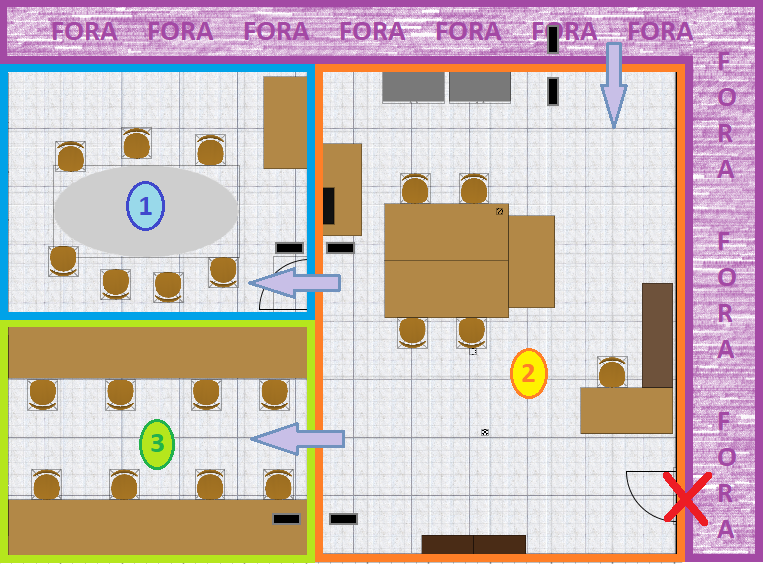
\includegraphics[width=0.9\linewidth]{figs/Metodologia/LARA_planta_ambientes.png}
    \caption{Imagem apresentando a planta baixa do LARA - local de instalação das leitoras}
    \label{fig:LARA_planta}
\end{figure}

O ambiente do laboratório pode ser melhor visualizado nas figuras \ref{fig:LARA1} e \ref{fig:LARA2} abaixo. As figuras mostram as projeções tridimensionais do laboratório, a partir de dois pontos de vista diferentes, para melhor compreensão do ambiente de estudo.

  \begin{figure}[H]
    \centering
    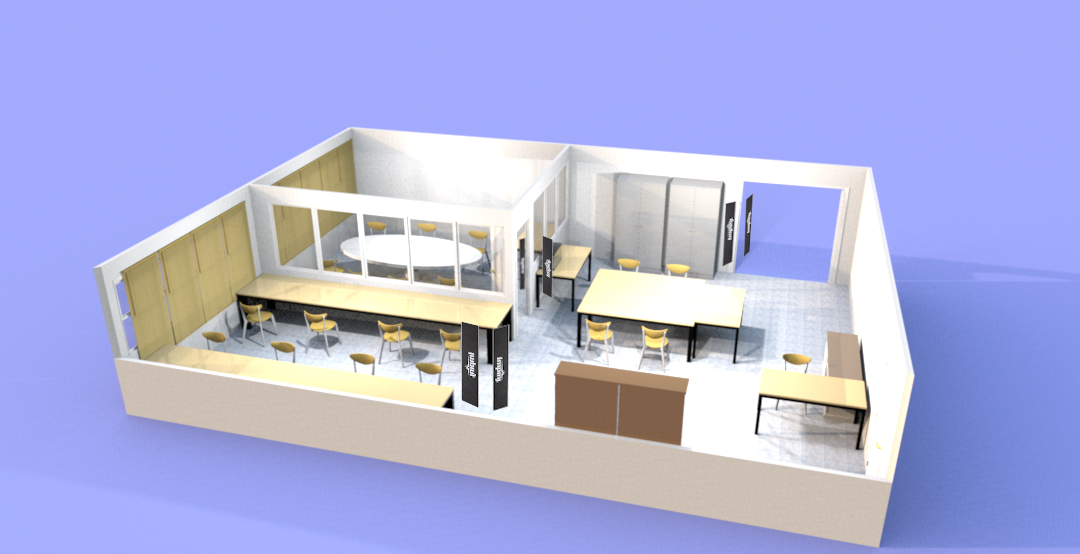
\includegraphics[width=1\linewidth]{figs/Metodologia/LARA_leitoras-1.png}
    \caption{Imagem apresentando a renderização tridimensional do LARA e o local de instalação das leitoras}
    \label{fig:LARA1}
\end{figure}

  \begin{figure}[H]
    \centering
    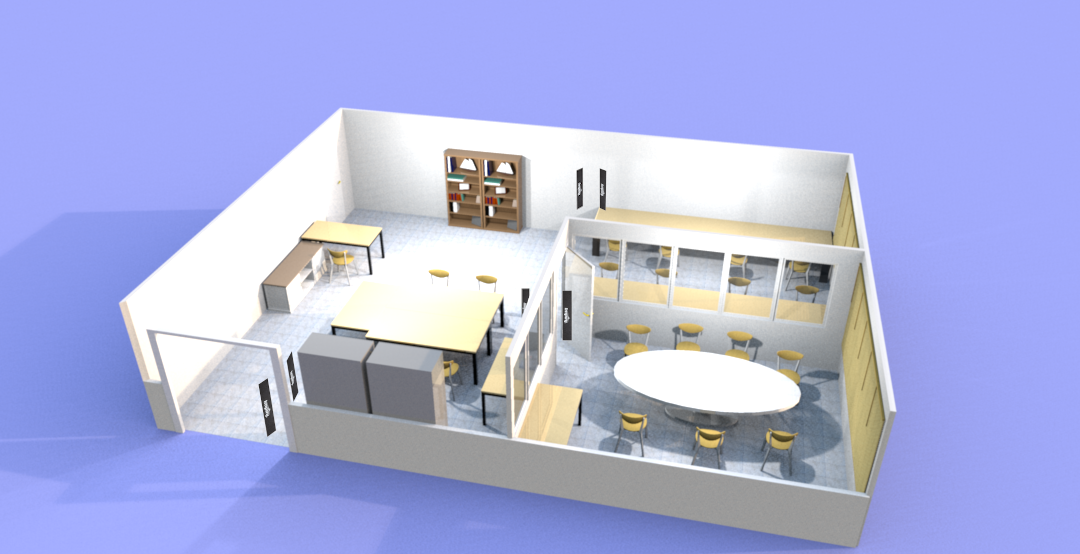
\includegraphics[width=1\linewidth]{figs/Metodologia/LARA_leitoras-2.png}
    \caption{Imagem apresentando a renderização tridimensional do LARA a partir de um segundo ponto de vista - local de instalação das leitoras}
    \label{fig:LARA2}
\end{figure}

As três leitoras foram designadas para tratar os dados das transições. A leitora 1 (L1) trata os dados da transição entre o Ambiente Externo (0) e a Sala Principal (1); a Leitora 2 (L2) é responsável por capturar os dados da transição entre a Sala Principal (1) e a Sala de Reuniões (2); a Leitora 3 registra os cartões que passam pela transição entre a Sala Principal (1) e o Corredor de Baias (3). Cada leitora é representada por um retângulo cinza na figura \ref{fig:LARA_planta} e possui duas antenas para registrar as \textit{tags} que passam na região.

As antenas foram dispostas em locais estratégicos para se obter as leituras mais precisas, nos locais de transição de interesse. Estes locais estão localizados próximos às portas ou passagens onde estão as fronteiras dos ambientes definidos. As antenas podem ser vistas como retângulos pretos de borda cinza na figura \ref{fig:LARA_planta} e pelo desenho da leitora real nas figuras \ref{fig:LARA1} e \ref{fig:LARA1}.

As leitoras da transição entre os ambientes Sala Principal (1) e Sala de Reuniões (2) e da transição entre os ambientes Sala Principal (1), Corredor de Baias (3) foram instaladas em posições opostas da sala para minimizar a ocorrência de leitura das \textit{tags} pelas duas leitoras ao mesmo tempo.

 \subsection{Elaboração do Software}
 
 A tecnologia RAIN RFID, geralmente utilizada para aplicações de \textit{IoT} (Internet das coisas - \textit{Internet of Things} em inglês), exige a implementação de um \textit{middleware} para conectar os dados crus das TAGs registrados pelas leitoras RFID às aplicações de alto nível e de computação em nuvem, como pode ser observado na figura \ref{fig:RFID-Middleware} do capítulo anterior, sessão \ref{section: middleware}. Por esse motivo, o pacote OctaneSDK da Impinj foi escolhido para implementar a aplicação de localização de pessoas. O pacote possui classes prontas de comunicação e configuração das leitoras Impinj Speedway R420 usadas. Será considerado, portanto, que o programa criado não se trata de um \textit{middleware}, mas de uma aplicação apenas, mesmo executando tarefas de comunicação com as leitoras.
 
 O \textit{software} elaborado simula internamente o ambiente do LARA como uma Rede de Petri, onde cada estado da rede representa um ambiente do LARA enquanto cada transição representa um par de antenas instaladas nas portas ou passagens. Os marcadores da Rede de Petri representam as TAGs das pessoas, transitando livremente pelos ambientes e transições. Um modelo que representa o funcionamento do programa pode ser visto na figura \ref{fig:Petri1}.
 
 \begin{figure}[H]
    \centering
    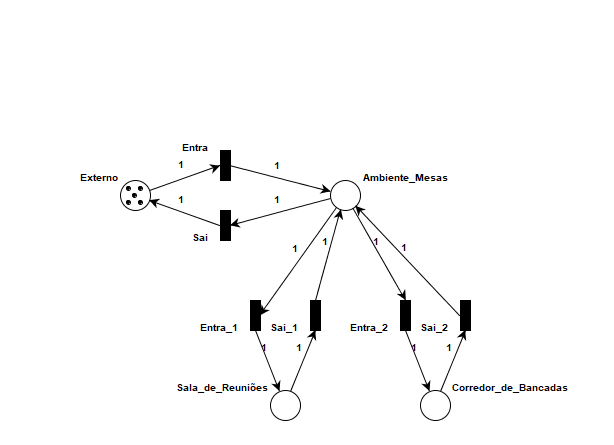
\includegraphics[width=0.8\linewidth]{figs/Metodologia/Petri_net.png}
    \caption{Rede de Petri representando todas as possibilidades circulação de pessoas pelo LARA como estados e transições}
    \label{fig:Petri1}
\end{figure}

Simulando a Rede de Petri é possível observar a ideia da circulação das pessoas pelo espaço do laboratório, onde cada transição ativada leva um marcador de um estado a outro, o que corresponde a uma pessoa cruzando uma fronteira para ir de um ambiente a outro. A figura \ref{fig:Petri2} mostra uma situação imaginária onde cinco pessoas transitam pelo laboratório. As transições marcadas em vermelho são as transições possíveis a partir do estado atual. A situação apresentada mostra duas pessoas na Sala Principal (1), duas pessoas na Sala de Reuniões (2) e uma pessoa no Corredor de Baias (3).

 \begin{figure}[H]
    \centering
    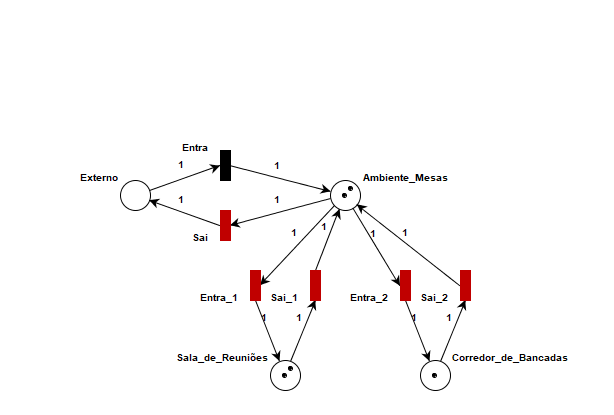
\includegraphics[width=0.8\linewidth]{figs/Metodologia/Petri_net2.png}
    \caption{Rede de Petri representando a circulação de pessoas pelo LARA em um caso hipotético}
    \label{fig:Petri2}
\end{figure}
 
 O programa criado em linguagem de programação C\# é orientado a objeto e cria as seguintes classes:
 
 \begin{itemize}
     \item \textbf{Programa:} contém a função \textit{main} e as funções básicas de configuração, comunicação e leituras;
     \item \textbf{Ambiente:} possui um nome, pode ter pessoas (\textit{cardholders}) e possui uma carga térmica associada à quantidade de pessoas em seu interior;
     \item \textbf{Pessoa (\textit{Cardholder}):} possui um nome, uma TAG (o número EPC associado à TAG) e uma carga térmica. Guarda a informação do ambiente em que se encontra e das curvas de histórico de leituras de valores RSSI e frequência Doppler;
     \item \textbf{Curva:} armazena os últimos $n$ valores de RSSI ou frequência Doppler, assim como o horário das leituras em que se capturaram essas informações;
     \item \textbf{Antena:} possui um número e está associada a uma leitora;
     \item \textbf{Transição:} conecta dois ambientes, e monitora duas antenas;
     \item \textbf{Projeto:} implementa os critérios de decisão de transição e registra as mudanças de ambiente dos \textit{cardholders};
     \item \textbf{Gerenciador de arquivos (\textit{FileHandler}):} Organiza e registra os dados coletados em arquivos CSV.
 \end{itemize}
 
 \subsection{Configuração das Leitoras}

 \begin{figure}[H]
    \centering
    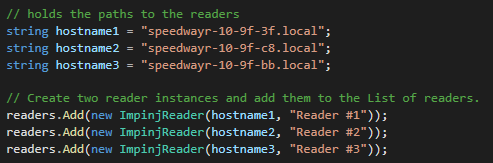
\includegraphics[width=0.8\linewidth]{figs/Metodologia/set_readers.PNG}
    \caption{Comandos de linha de código para estabelecer as leitoras}
    \label{fig:set_readers}
\end{figure}

 \begin{figure}[H]
    \centering
    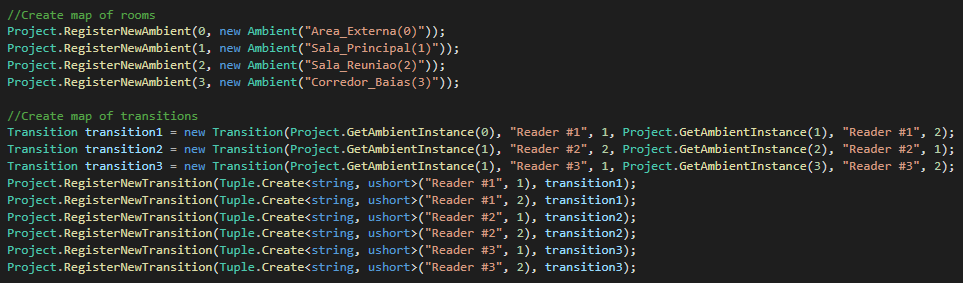
\includegraphics[width=1\linewidth]{figs/Metodologia/set_rooms&transitions.PNG}
    \caption{Comandos de linha de código para estabelecer os ambientes e as transições}
    \label{fig:set_AmbTran}
\end{figure}

 \begin{figure}[H]
    \centering
    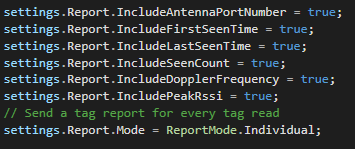
\includegraphics[width=0.6\linewidth]{figs/Metodologia/report_settings.PNG}
    \caption{Comandos de linha de código para configurar o modo de \textit{report} das leitoras}
    \label{fig:report_settings}
\end{figure}

 \begin{figure}[H]
    \centering
    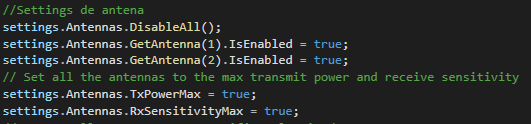
\includegraphics[width=0.8\linewidth]{figs/Metodologia/antenna_settings.PNG}
    \caption{Comandos de linha de código para configurar o modo de operação das antenas}
    \label{fig:antenna_settings}
\end{figure}

 \begin{figure}[H]
    \centering
    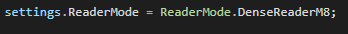
\includegraphics[width=0.6\linewidth]{figs/Metodologia/readermode_settings.PNG}
    \caption{Comando de linha de código para configurar o modo de operação das leitoras}
    \label{fig:readermode_settings}
\end{figure}


\textcolor{red}{TO BE CONTINUED} %TODO

 \subsection{Transições}
 
 Com o intuito de definir com a maior precisão possível o momento de passagem de uma pessoa de um ambiente para outro foi decidido monitorar as portas e passagens com duas antenas. O objetivo é acumular dados de potência de \textit{backscattering} das TAGs (RSSI) para possuir um valor comparativo de proximidade da TAG para cada antena. Além do sinal de potência RSSI, também é coletada a frequência de efeito Doppler, que indica um valor proporcional a velocidade vetorial em direção ortogonal à leitora, e pode indicar se a pessoa se aproxima ou de afasta desta.
 
 Durante testes preliminares, o analisou-se a variação dos valores de RSSI e frequência Doppler com uma única TAG e uma única antena. Os resultados deste teste podem ser encontrados na seção \ref{sect:testepreliminar}. Com base nesses resultados duas conclusões foram tiradas: as leituras de frequência de efeito Doppler podem ser facilmente divididas entre aproximação e afastamento de uma determinada antena e as leituras de potência RSSI aumentam proporcionalmente com a proximidade da TAG à antena, e diminuem proporcionalmente ao afastamento.
 
 A partir dessa ideia foi criado o conceito de transição, onde duas antenas registram a passagem de uma pessoa, e comparam entre si os dados RSSI e de frequência Doppler para estimar o sentido do caminhar da pessoa (entrando ou saindo de um ambiente). Cada antena fica de um lado da fronteira (porta ou passagem).
 
 Definindo-se o maior valor de RSSI durante todas as leituras na passagem de uma pessoa por uma fronteira, define-se esse como o momento em que a pessoa está mais próxima daquela antena. Realiza-se o mesmo procedimento para a segunda antena, do outro lado da fronteira. O ponto médio define o momento de transição de um ambiente para o outro. Da mesma forma, o momento em que uma pessoa deixa de aproximar-se e passa a se afastar de uma antena, este é o momento em que a pessoa está mais próxima da antena. Utilizando o mesmo critério do RSSI, o ponto médio entre o cruzamento na frente das duas antenas marca o momento de transição.
 
 \subsubsection{Curvas}
 
 Foram criados dois \textit{buffers} para armazenar as últimas leituras de cada TAG. Cada um armazena uma lista ordenada de tuplas $<x,y>$, onde $x$ é o tempo da leitura, e $y$ é a magnitude. A lista é ordenada com base na chave $x$, para garantir que os dados são salvos em ordem cronológica. O primeiro \textit{buffer} armazena as leituras de RSSI. O segundo armazena as leituras de frequência Doppler.Os \textit{buffers} foram chamados de "curvas", por guardarem as curvas históricas das últimas $n$ leituras para cada valor.
 
 O tamanho das curvas, inicialmente foi definido em 100 valores. Este se mostrou um valor demasiado grande, pois armazena dados de mais de uma passagem anterior, e atrapalha a análise dos dados. Definiu-se então que as curvas armazenariam 5 a 20 valores, padronizado em 12 leituras, por ser a faixa do tamanho médio da quantidade de leituras feitas em uma passagem a passos curtos em velocidade constante na frente das antenas.
 
 Após encher o \textit{buffer}, cada próxima leitura será armazenada no final da lista, após a retirada do primeiro elemento, tornando o \textit{buffer} uma fila.

 
 \subsection{Casos de teste}
 \textcolor{red}{TO BE CONTINUED} %TODO
 
  \begin{figure}[H]
    \centering
    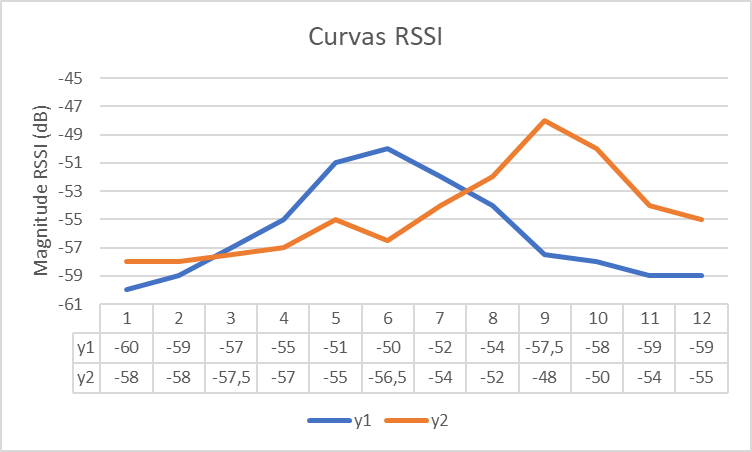
\includegraphics[width=0.8\linewidth]{figs/Metodologia/image001.png}
    \caption{Exemplo de curvas RSSI com dados gerados artificialmente}
    \label{fig:rssicurvesmet1}
\end{figure}

 \begin{figure}[H]
    \centering
    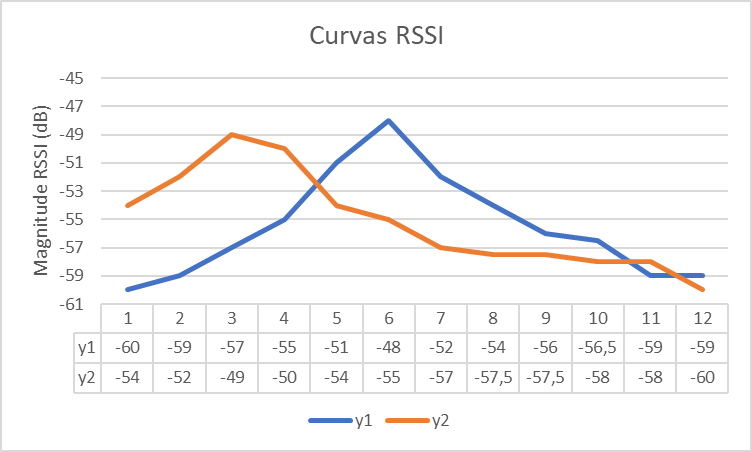
\includegraphics[width=0.8\linewidth]{figs/Metodologia/image005.png}
    \caption{Exemplo de curvas RSSI com dados gerados artificialmente}
    \label{fig:rssicurvesmet2}
\end{figure}

  \begin{figure}[H]
    \centering
    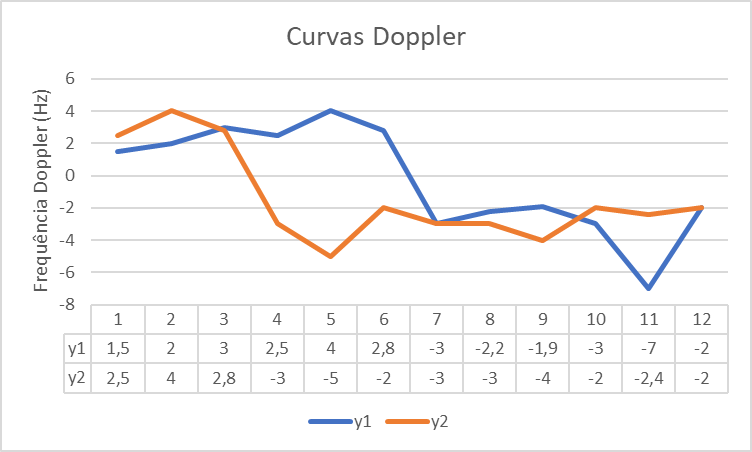
\includegraphics[width=0.8\linewidth]{figs/Metodologia/image003.png}
    \caption{Exemplo de curvas Doppler com dados gerados artificialmente}
    \label{fig:doppler_MET}
\end{figure}

 \begin{figure}[H]
    \centering
    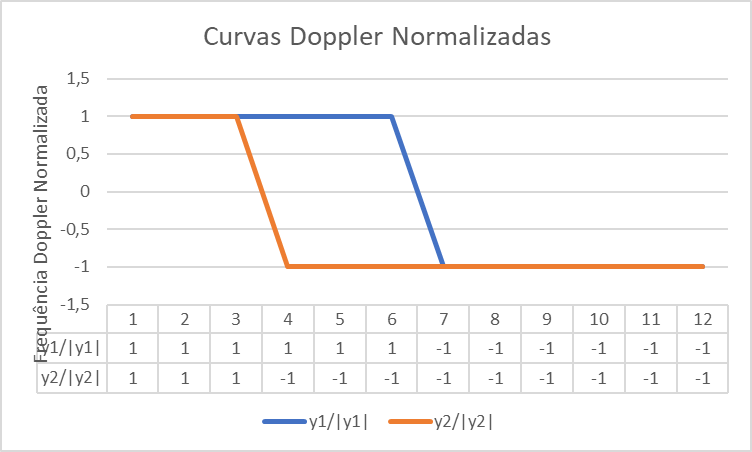
\includegraphics[width=0.8\linewidth]{figs/Metodologia/image007.png}
    \caption{Exemplo de curvas Doppler normalizado com dados gerados artificialmente}
    \label{fig:Doppler_norm_MET}
\end{figure}
 
 \subsubsection{Comparando a magnitude do último valor de RSSI capturado}
 
 \subsubsection{Comparando o tempo e magnitude dos picos das curvas de RSSI}
 
 \subsection{Comparando o tempo dos pontos de transição Doppler}
 
 \subsection{Combinando o critério de picos RSSI e transições Doppler}

